\documentclass{article}
\usepackage{amsmath}
\usepackage{amssymb}
\DeclareMathOperator{\Ima}{Im}
\DeclareMathOperator{\Hom}{Hom}

\section*{Solutions for chapter 2}

\subsection*{2.1}

\subsubsection*{2.1.1.2}
\usepackage{tikz}
\begin{document}
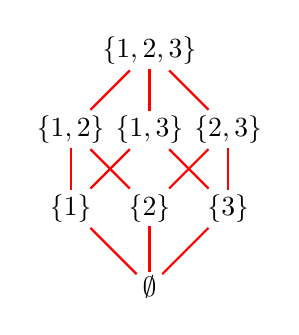
\begin{tikzpicture}
  \node (s) at (0, 0) {$\{1, 2, 3\}$};
  \node (s1) at (-1, -1) {$\{1, 2\}$};
  \node (s2) at (0, -1) {$\{1, 3\}$};
  \node (s3) at (1, -1) {$\{2, 3\}$};
  \draw [red,  thick, shorten <=-2pt, shorten >=-2pt] (s1) to (s);
  \draw [red, thick, shorten <=-2pt, shorten >=-2pt] (s2) to (s);
  \draw [red, thick, shorten <=-2pt, shorten >=-2pt] (s3) to (s);
  \node (s4) at (-1, -2) {$\{1\}$};
  \draw [red,  thick, shorten <=-2pt, shorten >=-2pt] (s4) to (s1);
  \draw [red, thick, shorten <=-2pt, shorten >=-2pt] (s4) to (s2);
  \node (s5) at (0, -2) {$\{2\}$};
  \draw [red,  thick, shorten <=-2pt, shorten >=-2pt] (s5) to (s1);
  \draw [red,  thick, shorten <=-2pt, shorten >=-2pt] (s5) to (s3);
  \node (s6) at (1, -2) {$\{3\}$};
  \draw [red,  thick, shorten <=-2pt, shorten >=-2pt] (s6) to (s2);
  \draw [red,  thick, shorten <=-2pt, shorten >=-2pt] (s6) to (s3);
  \node (s7) at (0, -3) {$\emptyset$};
  \draw [red,  thick, shorten <=-2pt, shorten >=-2pt] (s7) to (s4);
  \draw [red,  thick, shorten <=-2pt, shorten >=-2pt] (s7) to (s5);
  \draw [red,  thick, shorten <=-2pt, shorten >=-2pt] (s7) to (s6);
\end{tikzpicture}

\subsubsection*{2.1.2.2}
The connection pattern constitutes a function $PR \to RG$.

\subsubsection*{2.1.2.3}
$\Ima(f) = {y_{1}, y_{2}, y_{4}}$.

\subsubsection*{2.1.2.4}
$\lvert \Hom_{\boldsymbol{Set}}\left(A, B\right) \rvert =2^{5}$,
$\lvert \Hom_{\boldsymbol{Set}}\left(B, A\right) \rvert = 5^{2}$

\subsubsection*{2.1.2.5} \label{problem-2125}
Let $A = \{*\}$, the single point set. Then for any set $X$, there is
only one mapping that takes $X$ to $A$, the map $x\mapsto*$, $x \in
X$. Let $B = \emptyset$. Then for all sets $X$, there is only one
mapping that takes $B$ to $X$, the empty function $f_{X} : \emptyset
\to X$.

\subsubsection*{2.1.2.9}
$n!$ for $n \ge 0$. In the case $n = 0$, there is one isomorphism (the
empty function of the last problem).

\subsubsection*{2.1.2.12}
Take $A = \{*\}$. Then $\Hom_{\boldsymbol{Set}}\left(A, X \right)$ is
the set of constants in $X$.  The isomporphism itself is, with $x \in
X$, $(* \to x) \to x$.

\clearpage

\subsubsection*{2.1.2.13}
$f(4) = c$.\\
$s$ as a sequence is $\left(1, 4, 9, 16, 25, 36, 49\right)$.

\subsubsection*{2.1.2.15}
$\lvert A \rvert = 3$,$\lvert \mathbb{N} \rvert \ge \infty $, $\lvert
\{n \in \mathbb{N}\;|\; n \le 5\}\rvert = 6$.

\end{document}
